\documentclass{article}

%===============================
%
%          📦 Paquetes
%
%===============================

% === Configuración del documento y tipografía ===
\usepackage[a4paper, top=3cm, bottom=2.5cm, left=2.5cm, right=2.5cm]{geometry}
\usepackage[spanish]{babel}
\usepackage[utf8]{inputenc}
\usepackage[T1]{fontenc}
\usepackage{eulervm}



% === Gráficos y representaciones visuales ===
\usepackage{tikz}
\usepackage{pgfplots}
\pgfplotsset{compat=1.18}
\usepackage{graphicx}
\usepackage{subcaption}

% === Estilo y personalización ===
\usepackage{titling}
\usepackage{titlesec}
\usepackage{tocloft} 
\usepackage{fancyhdr}
\usepackage{setspace}
\usepackage{caption}

% === Matemáticas y símbolos ===
\usepackage{amsmath}
\usepackage{amssymb}
\usepackage{cancel}

% === Estructura y disposición del contenido ===
\usepackage{array}
\usepackage{multicol}
\usepackage{float}
\usepackage{indentfirst}

% === Hipervínculos y referencias ===
\usepackage{tocbibind}
\usepackage[colorlinks=true, linkcolor=black]{hyperref}

%===============================
%
%          ⬆️⬇️ Cabeceras
%
%===============================
\pagestyle{fancy}
\fancyhf{}
\fancyhead[L]{
\includegraphics[width=2.5cm,clip,trim=0cm 1cm 24cm 1cm]{assets/logo-utp.png}}
\vspace{0.5mm}\fancyhead[R]{\textit{Gestión de Proyectos}\vspace{0.5mm}}
\fancyfoot[R]{\thepage}
\setlength{\headheight}{26.23502pt}
\addtolength{\topmargin}{-5.64944pt}

%======================================
%
%          📑 Espaciado de Párrafos
%
%======================================

\setlength{\parskip}{1.5em}
\setlength{\parindent}{0pt}

%===============================
%
%          📕 Estructura del título
%
%======================================
\title{
  \pagenumbering{gobble}
  \vspace{1cm}
  % 
\includegraphics[width=5cm,clip,trim=6cm 6cm 6cm 6cm]{./assets/isotipo.jpg} \\
  
\includegraphics[width=5cm,clip,trim=0cm 2.9cm 0cm 0cm]{./assets/isotipo-utp.png} \\
  \vspace{0.5cm}
  \textbf{Universidad Tecnológica del Perú} \\
  \vspace{0.5cm}
  \text{Gestión de Proyectos} \\
  \vspace{1cm}
    {\huge \textbf{(AC-S09) Avance de Proyecto Final 1 (APF1)}} \\
  \vspace{1cm}
  % \large \textbf{Para acceder al título de...} \\
}
\author{
  \begin{tabular}{ll}
    \textbf{Huatay Salcedo, Luis Elías, \texttt{U71809640}}\\
    % \textbf{Huatay Salcedo, Luis Elías, \texttt{U71809640}}\\
  \end{tabular} \\
  % \texttt{Ingeniería}\\
}
\begin{document}
% \date{14 de agosto de 2024}
\maketitle
\begin{center}
  Docente: \textbf{Rogelio Chambi Oscco} \\
\end{center}

%======================================
%
%          📚 Inicio del documento
%
%======================================

\newpage

\begin{center}
\Large\bfseries Índice
\end{center}
\begingroup
\let\clearpage\relax
\renewcommand{\contentsname}{}
\tableofcontents
\endgroup


\newpage
% Inicio de la numeración de páginas (desde aquí)
\pagenumbering{arabic}
\setcounter{page}{1}  
\vspace*{\fill}

\section{Introducción}

  El presente proyecto tiene como finalidad aplicar la Metodología de Gestión de Proyectos Clásica, siguiendo el marco de trabajo propuesto por el Project Management Institute (PMI) y utilizando herramientas del Framework del PMBOK. Durante la primera parte de la unidad, se desarrollará un marco predictivo para la gestión de un proyecto empresarial, abarcando las fases de Iniciación y Planificación.

  Para ello, se seleccionará una empresa y área específica, describiendo su misión, visión y objetivos estratégicos, así como el alineamiento del proyecto con dichos objetivos. Posteriormente, se documentarán los procesos de iniciación (objetivos, alcance inicial, gestión de interesados y acta de constitución) y planificación (gestión de integración, alcance, cronograma, costes, calidad, recursos, comunicaciones, riesgos y adquisiciones).

  Finalmente, se presentará un informe detallado que incluya todos los elementos mencionados, demostrando la capacidad de aplicar la metodología de gestión de proyectos en un entorno empresarial real.

\vspace*{\fill}

\section{Descripción de la empresa y Área afectada por el proyecto a implementar}

\subsection{Nombre de la empresa y/o Área}
\textbf{Empresa:} Global GIS Service (GGS) \\
\textbf{Área afectada:} Investigación y Desarrollo (I+D)

\subsection{Misión y Visión de la empresa}

\textbf{Misión:} \\
Desarrollar soluciones geoespaciales innovadoras que optimicen la toma de decisiones estratégicas en organizaciones públicas y privadas, integrando tecnología GIS con metodologías ágiles y sostenibles.

\textbf{Visión:} \\
Ser líderes en Latinoamérica en el desarrollo de plataformas GIS interoperables, escalables y centradas en el usuario, contribuyendo a la transformación digital del sector educativo, gubernamental y empresarial.

\subsection{Objetivos Estratégicos de la empresa y/o Área}

\textbf{Objetivos Estratégicos de Global GIS Service (GGS):}
\begin{itemize}
    \item Expandir la adopción de soluciones GIS en sectores clave como educación, gobierno y servicios públicos.
    \item Garantizar la interoperabilidad entre plataformas GIS y sistemas de terceros.
    \item Fortalecer la relación con clientes mediante procesos de validación colaborativos y comunicación efectiva.
    \item Promover la capacitación continua de usuarios finales para asegurar el uso eficiente de las soluciones implementadas.
\end{itemize}

\textbf{Objetivos Estratégicos del Área de I+D:}
\begin{itemize}
    \item Diseñar una metodología de trabajo sostenible y replicable para el desarrollo de proyectos GIS.
    \item Fomentar la innovación mediante la incorporación de tecnologías emergentes en los procesos de desarrollo.
    \item Asegurar la calidad técnica de los entregables a través de revisiones periódicas y pruebas de integración.
    \item Generar conocimiento interno que permita escalar soluciones de manera eficiente en nuevos mercados.
\end{itemize}

\subsection{Alineamiento del proyecto con los objetivos de la empresa}

El proyecto \textbf{Global GIS Service GGS} se alinea directamente con los objetivos estratégicos de la empresa y del área de I+D en los siguientes aspectos:

\begin{itemize}
    \item \textbf{Interoperabilidad tecnológica:} El proyecto aborda la integración entre plataformas GIS y sistemas del cliente, lo cual responde al objetivo de garantizar compatibilidad y escalabilidad.
    \item \textbf{Metodología sostenible:} La implementación de sesiones prácticas, manuales claros y validaciones técnicas contribuye a establecer una metodología de trabajo replicable en futuros proyectos.
    \item \textbf{Gestión del conocimiento:} Las reuniones técnicas mensuales y los informes especializados permiten documentar aprendizajes y buenas prácticas, fortaleciendo el capital intelectual del área de I+D.
    \item \textbf{Transformación digital:} Al automatizar procesos de validación, capacitación y comunicación, el proyecto impulsa la digitalización de la gestión geoespacial en el cliente, alineándose con la visión de liderazgo regional en soluciones GIS.
\end{itemize}


\section{Proceso de Iniciación}

En el proceso de inicación, se definen los objetivos del proyecto, su alcance inicial, la gestión de interesados y se elabora el acta de constitución del proyecto. Esto establece las bases para la planificación y ejecución del mismo.

\subsection{Objetivos del Proyecto}
\begin{itemize}
    \item Implementar una solución GIS interoperable que permita integrar plataformas geoespaciales con los sistemas del cliente.
    \item Establecer una metodología de trabajo sostenible y replicable para futuros desarrollos GIS desde el área de I+D.
    \item Mejorar la calidad de los datos y la eficiencia operativa mediante validaciones técnicas y automatización de procesos.
    \item Fortalecer la relación con el cliente a través de una comunicación efectiva y validación continua de entregables.
\end{itemize}

\subsection{Alcance Inicial del Proyecto}

El proyecto \textbf{Global GIS Service GGS} tiene como alcance inicial el diseño e implementación de servicios de consultoría en Sistemas de Información Geográfica (GIS) para clientes en sectores público y privado. El alcance incluye:
\begin{itemize}
    \item Análisis de necesidades y requisitos del cliente.
    \item Desarrollo de soluciones GIS personalizadas.
    \item Integración de plataformas GIS con sistemas existentes del cliente.
    \item Capacitación básica a usuarios finales.
    \item Documentación técnica y manuales de usuario.
\end{itemize}

\subsubsection{Registro de Interesados}

\begin{table}[H]
\centering
\renewcommand{\arraystretch}{1.3}
\begin{tabular}{|p{4cm}|p{10cm}|}
\hline
\textbf{Atributo} & \textbf{Valores} \\
\hline
Rol en Proyecto & Patrocinador, Especialista Técnico \\
\hline
Nombre & Dra. Rosmery R., Ing. Marco T. \\
\hline
Cargo & Directora de Investigación y Proyectos Estratégicos, Especialista GIS \\
\hline
Área & Dirección, Área Técnica \\
\hline
Principal Requerimiento & Alineación estratégica del proyecto con los objetivos institucionales, Interoperabilidad entre plataformas GIS y sistemas del cliente \\
\hline
Influencia (Poder / Interés) & Alta / Alta, Media / Alta \\
\hline
Estrategia & Reuniones periódicas, reportes ejecutivos, validación de entregables; Involucramiento en revisiones técnicas, pruebas de integración \\
\hline
¿Aprueba Alcance / Plan? & Sí, No \\
\hline
Anexo & A1, A2 \\
\hline
Contacto & 999-123-456, 999-987-654 \\
\hline
\end{tabular}
\caption{Registro de Interesados del Proyecto Global GIS Service GGS (orientación horizontal)}
\end{table}

\subsubsection{Acta de Constitución del Proyecto}

\begin{table}[H]
\centering
\renewcommand{\arraystretch}{1.4}
\begin{tabular}{|p{5cm}|p{10cm}|}
\hline
\textbf{Componente} & \textbf{Descripción} \\
\hline
Equipo & Global GIS Service GGS \\
\hline
Nombre del Proyecto & Consultoría Integral en Soluciones GIS \\
\hline
Gerente del Proyecto & Luis Huatay – Nivel de autoridad: Alto. Reporta a la Dirección de Proyectos Estratégicos. Pertenece a Global GIS Service. \\
\hline
Patrocinador del Proyecto & Dra. Rosmery R. – Directora de Investigación y Proyectos Estratégicos \\
\hline
Descripción del Proyecto & Diseño e implementación de servicios de consultoría especializados en Sistemas de Información Geográfica (GIS), orientados a mejorar la toma de decisiones mediante análisis espacial, interoperabilidad tecnológica y capacitación de usuarios. \\
\hline
Justificación del Proyecto & Alta demanda en sectores público y privado por soluciones geoespaciales integradas. Necesidad de posicionar a la empresa como referente regional en consultoría GIS. Oportunidad de generar ventajas competitivas mediante visualización de datos y transformación digital. \\
\hline
Objetivos del Proyecto y Criterios de Éxito & 
\begin{itemize}
    \item Brindar servicios GIS personalizados que satisfagan necesidades específicas (criterio: contratos ejecutados con éxito).
    \item Entregar soluciones en un plazo máximo de 8 semanas por cliente (criterio: cumplimiento del cronograma).
    \item Superar el 90\% de satisfacción del cliente en encuestas de cierre.
\end{itemize} \\
\hline
Requerimientos Principales (Alto nivel) & Plataformas GIS, personal especializado en análisis espacial y programación, documentación técnica, capacitación básica a usuarios finales. \\
\hline
Riesgos Principales (Alto nivel) & Interoperabilidad limitada entre sistemas GIS y plataformas del cliente, dependencia de datos externos, restricciones presupuestarias. \\
\hline
Resumen del Cronograma de Hitos & 
\begin{itemize}
    \item Septiembre - Octubre: Definición y constitución de la empresa.
    \item Noviembre - Diciembre: Desarrollo de la oferta de servicios y marketing inicial.
\end{itemize} \\
\hline
Presupuesto Resumido (Orden de Magnitud) & S/. 20,000 en 4 meses \\
\hline
Supuestos & Disponibilidad de datos geoespaciales confiables, colaboración activa de los clientes, acceso a infraestructura tecnológica mínima. \\
\hline
Restricciones & Presupuesto limitado, plazos ajustados, disponibilidad de personal especializado. \\
\hline
Interesados & Ingeniero de Software especializado en GIS, Directora de Investigación y Proyectos Estratégicos, PMO, usuarios finales, equipos técnicos del cliente. \\
\hline
Requerimientos de Aprobación del Proyecto & Aprobación formal del patrocinador y del equipo directivo. Validación del acta de constitución por unanimidad. \\
\hline
\end{tabular}
\caption{Acta de Constitución del Proyecto: Global GIS Service GGS}
\end{table}




\section{Planificación}

  En esta sección se detallan los procesos de planificación del proyecto, incluyendo la gestión de la integración, alcance, cronograma, costes, calidad, recursos, comunicaciones, riesgos y adquisiciones. Cada uno de estos aspectos es fundamental para asegurar que el proyecto se ejecute de manera eficiente y efectiva, alineándose con los objetivos estratégicos de la empresa.

    Se utilizarán herramientas y técnicas del PMBOK para desarrollar un plan de proyecto integral que guíe todas las fases posteriores del mismo. Esto incluye la definición clara del alcance del proyecto, la elaboración de un cronograma detallado con hitos clave, la estimación y control de costes, así como la identificación y mitigación de riesgos potenciales.

    Además, se establecerán mecanismos de comunicación efectivos para mantener informados a todos los interesados y asegurar una gestión adecuada de los recursos humanos y materiales necesarios para la ejecución del proyecto.

    \subsection{Gestión de la Integración del Proyecto}
    
    \textbf{Objetivo:}
      Coordinar de manera efectiva todos los componentes del proyecto, asegurando la coherencia entre los procesos de iniciación, planificación, ejecución, monitoreo, control y cierre, para cumplir con los objetivos estratégicos de la empresa.

      \textbf{Procesos Clave}
      \begin{itemize}
          \item \textbf{Desarrollar el Acta de Constitución del Proyecto:} Formaliza el inicio del proyecto y define los objetivos, alcance y responsables.
          \item \textbf{Desarrollar el Plan para la Dirección del Proyecto:} Integra los planes subsidiarios (alcance, cronograma, costos, calidad, riesgos, comunicaciones, interesados).
          \item \textbf{Dirigir y Gestionar el Trabajo del Proyecto:} Ejecuta las actividades planificadas, gestiona recursos, genera entregables y asegura la calidad.
          \item \textbf{Gestionar el Conocimiento del Proyecto:} Captura, comparte y reutiliza conocimiento tácito y explícito para mejorar resultados y fomentar el aprendizaje organizacional.
          \item \textbf{Monitorear y Controlar el Trabajo del Proyecto:} Supervisa el desempeño, identifica desviaciones y toma acciones correctivas.
          \item \textbf{Realizar el Control Integrado de Cambios:} Evalúa y aprueba cambios que afecten el alcance, tiempo, costo o calidad.
          \item \textbf{Cerrar el Proyecto o Fase:} Verifica la aceptación de entregables, documenta lecciones aprendidas y formaliza el cierre.
      \end{itemize}

      \textbf{Entradas Principales}
      \begin{itemize}
          \item Acta de Constitución del Proyecto
          \item Plan para la Dirección del Proyecto
          \item Documentos del Proyecto
          \item Factores Ambientales de la Empresa
          \item Activos de los Procesos de la Organización
      \end{itemize}

      \textbf{Herramientas y Técnicas}
      \begin{itemize}
          \item Juicio de Expertos
          \item Sistemas de Información para la Gestión del Proyecto
          \item Reuniones
          \item Gestión del Conocimiento e Información
          \item Habilidades Interpersonales: escucha activa, facilitación, liderazgo, creación de relaciones, conciencia política
      \end{itemize}

      \textbf{Salidas}
      \begin{itemize}
          \item Entregables
          \item Datos de Desempeño del Trabajo
          \item Solicitudes de Cambio
          \item Registro de Incidentes
          \item Actualizaciones al Plan para la Dirección del Proyecto
          \item Actualizaciones a los Documentos del Proyecto
          \item Actualizaciones a los Activos de los Procesos de la Organización
          \item Registro de Lecciones Aprendidas
      \end{itemize}

    \subsection{Gestión del Alcance del Proyecto}

    Se desarrolla la EDT, un EDT es una descomposición jerárquica del trabajo del proyecto que define y organiza el alcance total del proyecto. La EDT descompone el proyecto en componentes más pequeños y manejables, facilitando la planificación, ejecución y control del proyecto.

    \begin{figure}[H]
      \centering
      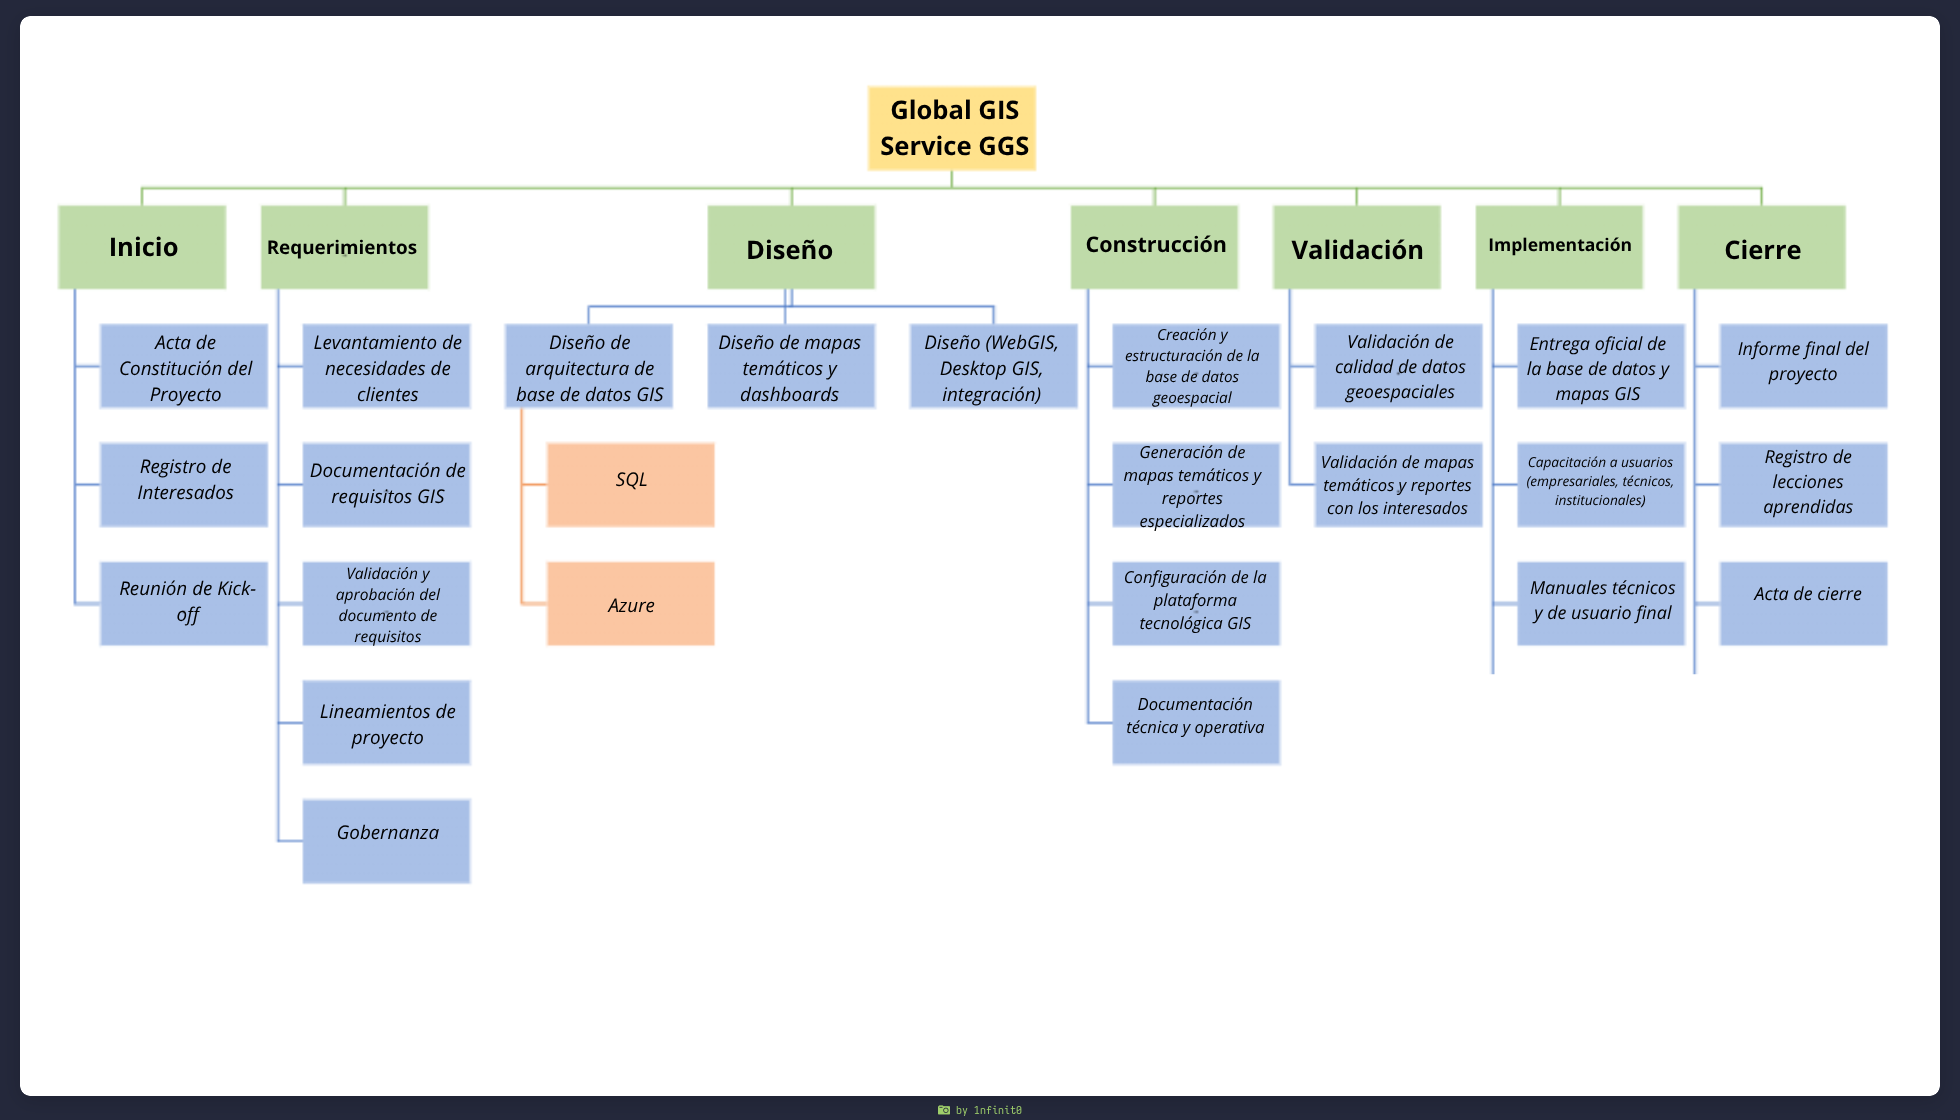
\includegraphics[width=1.5\textwidth,angle=90,trim=1cm 1cm 1cm 1cm,clip]{assets/EDT.png}
      \caption{Ejemplo de Estructura de Desglose del Trabajo (EDT) del proyecto.}
      \label{fig:edt}
    \end{figure}

    \subsubsection{Gestión del Cronograma del Proyecto}

    \textbf{Objetivo}
    Planificar, desarrollar, monitorear y controlar el cronograma del proyecto para asegurar el cumplimiento de los plazos establecidos, optimizando recursos y gestionando desviaciones de manera efectiva.

    \begin{multicols}{2}
      \textbf{Procesos Clave}
    \begin{itemize}
        \item \textbf{Planificar la Gestión del Cronograma:} Definir cómo se desarrollará, gestionará y controlará el cronograma.
        \item \textbf{Definir las Actividades:} Identificar las tareas específicas necesarias para producir los entregables del proyecto.
        \item \textbf{Secuenciar las Actividades:} Establecer el orden lógico de ejecución de las actividades.
        \item \textbf{Estimar la Duración de las Actividades:} Determinar el tiempo requerido para completar cada actividad.
        \item \textbf{Desarrollar el Cronograma:} Integrar actividades, duraciones, dependencias y recursos en un cronograma realista.
        \item \textbf{Controlar el Cronograma:} Monitorear el progreso, actualizar el cronograma y gestionar cambios a la línea base.
    \end{itemize}

    \textbf{Entradas}
    \begin{itemize}
        \item Plan para la Dirección del Proyecto
        \item Línea base del cronograma
        \item Documentos del proyecto (calendarios, estimaciones, riesgos)
        \item Datos de desempeño del trabajo
        \item Activos de los procesos de la organización
    \end{itemize}

    \textbf{Herramientas y Técnicas}
    \begin{itemize}
        \item Análisis de datos: valor ganado (SV, SPI), tendencias, variaciones, escenarios
        \item Método de la ruta crítica
        \item Sistema de información para la dirección de proyectos
        \item Optimización de recursos
        \item Adelantos y retrasos
        \item Compresión del cronograma
        \item Gráfica de trabajo pendiente por iteración
    \end{itemize}

    \textbf{Salidas}
    \begin{itemize}
        \item Informes de desempeño del trabajo
        \item Pronósticos del cronograma
        \item Solicitudes de cambio
        \item Actualizaciones al plan para la dirección del proyecto (línea base, costos, desempeño)
        \item Actualizaciones a los documentos del proyecto (cronograma, calendario de recursos, riesgos)
    \end{itemize}

    \textbf{Indicadores de Control}
    \begin{itemize}
        \item \textbf{SV (Schedule Variance):} Variación entre el trabajo planificado y el realizado.
        \item \textbf{SPI (Schedule Performance Index):} Índice de eficiencia temporal del proyecto.
        \item \textbf{Duración restante por actividad:} Estimación actualizada del tiempo requerido.
        \item \textbf{Gráfica de iteración:} Seguimiento visual del trabajo pendiente vs. ideal.
    \end{itemize}

    \end{multicols}

    \subsubsection{Gestión de los Costes del Proyecto}

      \begin{multicols}{2}
        \textbf{Objetivo}
        Planificar, estimar, controlar y actualizar los costos del proyecto para asegurar que se mantenga dentro del presupuesto aprobado, garantizando eficiencia financiera y toma de decisiones informada.

        \textbf{Procesos Clave}
        \begin{itemize}
            \item \textbf{Planificar la Gestión de Costes:} Definir cómo se estimarán, gestionarán y controlarán los costos del proyecto.
            \item \textbf{Estimar los Costos:} Determinar el costo aproximado de los recursos necesarios para completar cada actividad.
            \item \textbf{Determinar el Presupuesto:} Agregar los costos estimados para establecer una línea base de costos.
            \item \textbf{Controlar los Costos:} Monitorear el desempeño del proyecto frente a la línea base, gestionar desviaciones y actualizar proyecciones.
        \end{itemize}

        \textbf{Entradas}
        \begin{itemize}
            \item Plan para la Dirección del Proyecto
            \item Línea base de costos
            \item Requisitos de financiamiento del proyecto
            \item Documentos del proyecto (estimaciones, riesgos, supuestos)
            \item Datos de desempeño del trabajo
            \item Activos de los procesos de la organización
        \end{itemize}

        \textbf{Herramientas y Técnicas}
        \begin{itemize}
            \item Juicio de expertos
            \item Análisis de datos:
            \begin{itemize}
                \item Valor ganado (EV)
                \item Variación de costos (CV = EV - AC)
                \item Variación del cronograma (SV = EV - PV)
                \item Índice de desempeño del costo (CPI = EV / AC)
                \item Índice de desempeño del cronograma (SPI = EV / PV)
                \item Estimación a la conclusión (EAC)
                \item Estimación hasta la conclusión (ETC)
                \item Variación a la conclusión (VAC = BAC - EAC)
                \item Índice de desempeño del trabajo por completar (TCPI)
            \end{itemize}
            \item Sistema de información para la dirección de proyectos
            \item Análisis de tendencias y reservas
        \end{itemize}

        \textbf{Salidas}
        \begin{itemize}
            \item Informes de desempeño del trabajo
            \item Pronósticos de costos
            \item Solicitudes de cambio
            \item Actualizaciones al plan para la dirección del proyecto
            \item Actualizaciones a los documentos del proyecto (estimaciones, cronograma, riesgos)
            \item Registro de lecciones aprendidas
        \end{itemize}

        \textbf{Indicadores Clave}
        \begin{itemize}
            \item \textbf{EV (Valor Ganado):} Trabajo completado expresado en términos de presupuesto autorizado.
            \item \textbf{AC (Costo Real):} Costo incurrido por el trabajo realizado.
            \item \textbf{PV (Valor Planificado):} Presupuesto asignado al trabajo planificado.
            \item \textbf{CPI:} Eficiencia del costo. $CPI = \frac{EV}{AC}$
            \item \textbf{SPI:} Eficiencia del cronograma. $SPI = \frac{EV}{PV}$
        \end{itemize}
      \end{multicols}

    \subsubsection{Gestión de la Calidad del Proyecto}
      \begin{multicols}{2}
        \textbf{Objetivo}
Asegurar que los entregables del proyecto GIS cumplan con los requisitos técnicos, funcionales y de interoperabilidad definidos, garantizando la satisfacción del cliente y el cumplimiento de estándares internacionales de calidad.

\textbf{Procesos Clave}
\begin{itemize}
    \item \textbf{Planificar la Gestión de la Calidad:} Identificar los estándares de calidad aplicables al proyecto y documentar cómo se demostrará su cumplimiento.
    \item \textbf{Gestionar la Calidad:} Implementar actividades de mejora continua, revisión de procesos y validación técnica durante la ejecución del proyecto.
    \item \textbf{Controlar la Calidad:} Monitorear los entregables y procesos para verificar que cumplan con los requisitos establecidos, aplicando métricas y auditorías.
\end{itemize}

\textbf{Actividades de Calidad}
\begin{itemize}
    \item Validación de entregables principales por el comité de dirección.
    \item Revisión de pares del diseño del aplicativo por analistas expertos.
    \item Incorporación de controles de calidad en todos los procesos organizacionales.
    \item Auditoría del proyecto al cierre de la planificación.
\end{itemize}

\textbf{Métricas de Calidad}
\begin{itemize}
    \item Máximo de 40 errores por ciclo de prueba (supervisor de pruebas).
    \item Tiempo de respuesta inferior a 2 segundos por petición (supervisor técnico).
    \item Disponibilidad mínima del 95\% durante el primer año de uso.
    \item Nivel de satisfacción del cliente superior al 90\% en encuestas de cierre.
\end{itemize}

\textbf{Estándares y Referencias}
\begin{itemize}
    \item ISO 9000 – Definición de calidad como cumplimiento de requisitos.
    \item ISO 19115 y OGC – Estándares internacionales de geoinformación.
    \item Principios de Juran, Crosby y Deming sobre mejora continua y prevención.
\end{itemize}

\textbf{Consideraciones para Entornos Adaptativos}
\begin{itemize}
    \item Incorporación de revisiones frecuentes de calidad durante el ciclo de vida.
    \item Retrospectivas periódicas para identificar causas raíz y proponer mejoras.
    \item Validación temprana de entregables en lotes pequeños para reducir costos de corrección.
\end{itemize}

\textbf{Entradas, Herramientas y Salidas}
\textbf{Entradas:}
\begin{itemize}
    \item Acta de constitución del proyecto
    \item Plan para la dirección del proyecto
    \item Documentación de requisitos y matriz de trazabilidad
    \item Factores ambientales y activos de procesos organizacionales
\end{itemize}

\textbf{Herramientas y Técnicas:}
\begin{itemize}
    \item Juicio de expertos
    \item Análisis costo-beneficio y análisis de datos
    \item Reuniones, entrevistas y tormenta de ideas
    \item Diagramas de flujo, métricas de calidad, planificación de pruebas
\end{itemize}

\textbf{Salidas:}
\begin{itemize}
    \item Plan de gestión de la calidad
    \item Métricas de calidad
    \item Actualizaciones al plan para la dirección del proyecto
    \item Actualizaciones a los documentos del proyecto
    \item Registro de lecciones aprendidas
\end{itemize}

\textbf{Responsabilidades:}
\begin{itemize}
    \item El equipo de proyecto es responsable de la implementación de las actividades de gestión de la calidad.
    \item El líder de proyecto debe asegurar que se asignen los recursos necesarios para cumplir con los estándares de calidad.
    \item El comité de dirección debe validar y aprobar los entregables del proyecto.
\end{itemize}
      \end{multicols}

      \subsubsection{Gestión de los Recursos del Proyecto}

      \begin{multicols}{2}

\textbf{Objetivo}
Identificar, adquirir y gestionar los recursos humanos, técnicos y físicos necesarios para la ejecución exitosa del proyecto GIS, asegurando disponibilidad, eficiencia operativa y alineación con los objetivos estratégicos.

\textbf{Procesos Clave}
\begin{itemize}
    \item \textbf{Planificar la Gestión de Recursos:} Definir cómo se estimarán, asignarán y gestionarán los recursos del proyecto.
    \item \textbf{Adquirir Recursos:} Obtener los recursos físicos y humanos necesarios para ejecutar el trabajo del proyecto.
    \item \textbf{Desarrollar el Equipo:} Mejorar las competencias, interacción y ambiente del equipo para maximizar el desempeño.
    \item \textbf{Dirigir el Equipo:} Supervisar el desempeño, resolver conflictos y asegurar la motivación y compromiso del equipo.
    \item \textbf{Controlar los Recursos:} Asegurar que los recursos asignados se utilicen según lo planificado y gestionar ajustes cuando sea necesario.
\end{itemize}

\textbf{Tipos de Recursos}
\begin{itemize}
    \item \textbf{Humanos:} Gerente de Proyecto, Especialistas GIS, PMO, Analistas Técnicos, Capacitadores.
    \item \textbf{Tecnológicos:} Plataformas GIS (WebGIS, Desktop), servidores, software de análisis espacial.
    \item \textbf{Materiales:} Manuales impresos, equipos de capacitación, licencias de software (cuando aplican).
\end{itemize}

\textbf{Herramientas y Técnicas}
\begin{itemize}
    \item Juicio de expertos
    \item Asignación de roles y responsabilidades (matriz RACI)
    \item Evaluaciones de desempeño
    \item Reuniones de seguimiento y coaching
    \item Software de gestión de recursos y cronograma
\end{itemize}

\textbf{Salidas}
\begin{itemize}
    \item Registro de recursos
    \item Calendario de recursos
    \item Evaluaciones de desempeño
    \item Actualizaciones al plan para la dirección del proyecto
    \item Registro de lecciones aprendidas
\end{itemize}

\textbf{Consideraciones Estratégicas}
\begin{itemize}
    \item Asignación clara de roles para evitar saturación del equipo técnico.
    \item Capacitación continua para asegurar la calidad de los entregables.
    \item Gestión colaborativa para fomentar la innovación y el compromiso.
    \item Uso eficiente de recursos tecnológicos para garantizar interoperabilidad.
\end{itemize}

      \end{multicols}
\newpage
      \subsubsection{Gestión de las Comunicaciones del Proyecto}

      \begin{figure}[H]
        \centering
        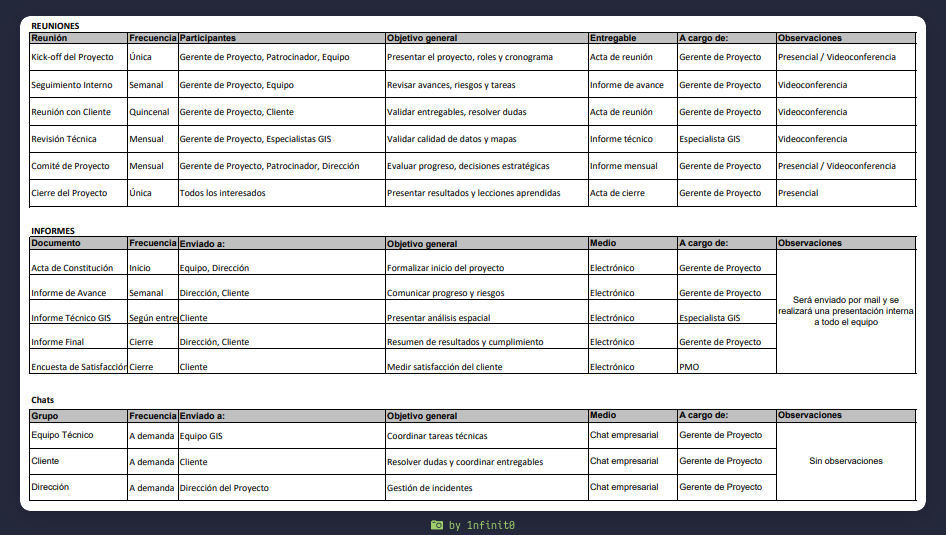
\includegraphics[width=1.3\textwidth,angle=90,trim=1cm 1cm 1cm 1cm,clip]{assets/comunicaciones.png}
        \caption{Diagrama de flujo de las comunicaciones del proyecto.}
        \label{fig:comunicaciones}
      \end{figure}

  \newpage

  \subsubsection{Gestión de los Riesgos del Proyecto}
  \begin{figure}[H]
        \centering
        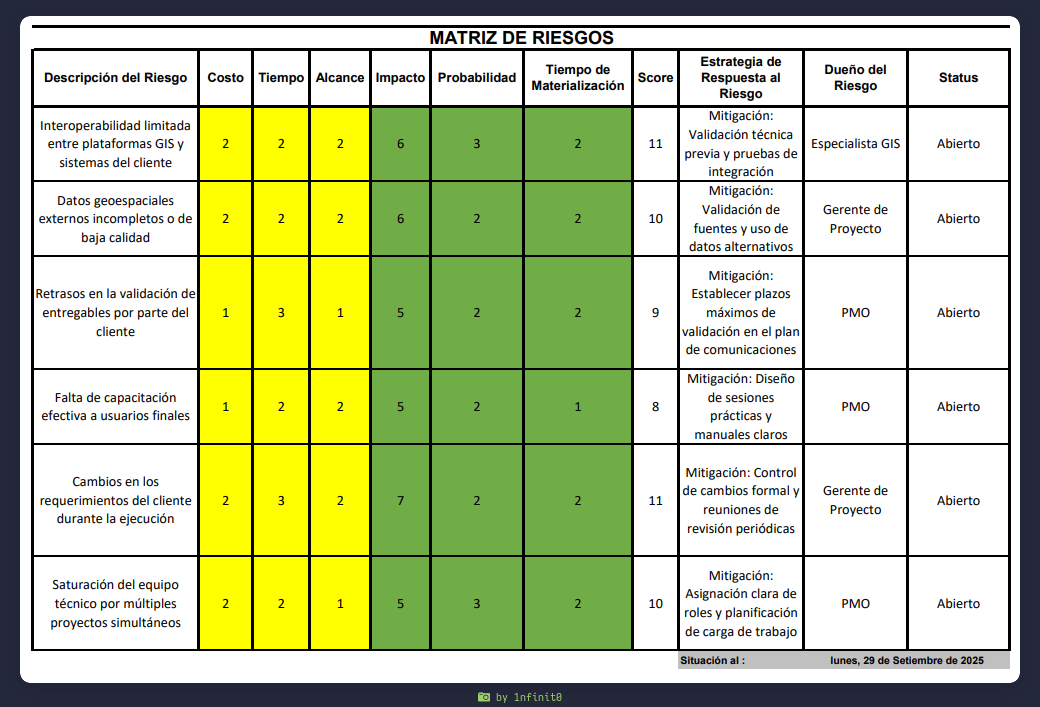
\includegraphics[width=1.3\textwidth,angle=90,trim=1cm 1cm 1cm 1cm,clip]{assets/riesgos.png}
        \caption{Diagrama de flujo de los riesgos del proyecto.}
        \label{fig:riesgos}
      \end{figure}

  \subsubsection{Gestión de las Adquisiciones del Proyecto}

\begin{multicols}{2}
  \textbf{Objetivo}
Gestionar de forma eficiente la compra de bienes, servicios y recursos externos necesarios para la ejecución del proyecto GIS, asegurando cumplimiento contractual, calidad técnica y optimización de costos.

\textbf{Procesos Clave}
\begin{itemize}
    \item \textbf{Planificar la Gestión de las Adquisiciones:} Identificar qué recursos deben ser adquiridos externamente, definir criterios de selección y establecer el enfoque contractual.
    \item \textbf{Efectuar las Adquisiciones:} Solicitar cotizaciones, evaluar proveedores, negociar contratos y formalizar acuerdos.
    \item \textbf{Controlar las Adquisiciones:} Supervisar el cumplimiento de los contratos, gestionar entregas, validar calidad y resolver incidencias.
\end{itemize}

\textbf{Bienes y Servicios Adquiribles}
\begin{itemize}
    \item Licencias de software GIS (cuando no se utilicen soluciones open source).
    \item Servicios de hosting y servidores para la plataforma WebGIS.
    \item Equipos de capacitación (proyectores, manuales impresos, estaciones de trabajo).
    \item Servicios especializados en análisis geoespacial o interoperabilidad (si no están disponibles internamente).
\end{itemize}

\textbf{Entradas}
\begin{itemize}
    \item Acta de constitución del proyecto
    \item Plan para la dirección del proyecto
    \item Requisitos técnicos y funcionales
    \item Presupuesto aprobado
    \item Políticas de compras de la organización
\end{itemize}

\textbf{Herramientas y Técnicas}
\begin{itemize}
    \item Juicio de expertos
    \item Análisis de mercado y proveedores
    \item Solicitud de propuestas (RFP) y cotizaciones (RFQ)
    \item Evaluación multicriterio
    \item Negociación contractual
    \item Sistema de información para la gestión de adquisiciones
\end{itemize}

\textbf{Salidas}
\begin{itemize}
    \item Contratos firmados
    \item Registro de adquisiciones
    \item Actualizaciones al plan para la dirección del proyecto
    \item Informes de desempeño de proveedores
    \item Registro de lecciones aprendidas
\end{itemize}

\textbf{Consideraciones Estratégicas}
\begin{itemize}
    \item Priorizar proveedores con experiencia en proyectos GIS y cumplimiento de estándares internacionales.
    \item Asegurar cláusulas de calidad, soporte técnico y propiedad intelectual en los contratos.
    \item Coordinar con el área de Finanzas para garantizar disponibilidad presupuestaria y trazabilidad.
    \item Documentar todo el proceso de adquisición para facilitar auditorías y futuras referencias.
\end{itemize}

\end{multicols}

\section{Conclusiones}

La gestión de adquisiciones en el proyecto GIS es fundamental para asegurar el acceso a los recursos necesarios y optimizar los costos. A través de una planificación adecuada, la selección de proveedores calificados y el control riguroso de los contratos, se puede garantizar el éxito del proyecto y la satisfacción de los interesados. La documentación y el aprendizaje continuo también son clave para mejorar los procesos en futuras iniciativas.

Los procesos de gestión de adquisiciones permiten una administración estructurada y eficiente, minimizando riesgos y asegurando que los recursos adquiridos cumplan con los requisitos técnicos y funcionales del proyecto. La colaboración estrecha con el equipo del proyecto y las áreas involucradas es esencial para alinear las adquisiciones con los objetivos estratégicos y operativos de la organización.

La gestión de adquisiciones no solo contribuye a la eficiencia operativa, sino que también fortalece la capacidad de la organización para llevar a cabo proyectos complejos en el futuro, estableciendo una base sólida para la mejora continua y la innovación en la gestión de proyectos GIS.




\end{document}